%\documentclass[preprint,10pt]{elsarticle}
\documentclass[review]{elsarticle}
%\documentclass[5p]{elsarticle} 

\usepackage{mathbf-abbrevs}

%\newcommand {\tbf}[1] {\textbf{#1}}
%\newcommand {\tit}[1] {\textit{#1}}
%\newcommand {\tmd}[1] {\textmd{#1}}
%\newcommand {\trm}[1] {\textrm{#1}}
%\newcommand {\tsc}[1] {\textsc{#1}}
%\newcommand {\tsf}[1] {\textsf{#1}}
%\newcommand {\tsl}[1] {\textsl{#1}}
%\newcommand {\ttt}[1] {\texttt{#1}}
%\newcommand {\tup}[1] {\textup{#1}}
%
%\newcommand {\mbf}[1] {\mathbf{#1}}
%\newcommand {\mmd}[1] {\mathmd{#1}}
%\newcommand {\mrm}[1] {\mathrm{#1}}
%\newcommand {\msc}[1] {\mathsc{#1}}
%\newcommand {\msf}[1] {\mathsf{#1}}
%\newcommand {\msl}[1] {\mathsl{#1}}
%\newcommand {\mtt}[1] {\mathtt{#1}}
%\newcommand {\mup}[1] {\mathup{#1}}

%some math functions and symbols
\newcommand{\reals}{{\mathbb R}}
\newcommand{\ints}{{\mathbb Z}}
\newcommand{\integers}{{\mathbb Z}}
\newcommand{\sign}[1]{\mathtt{sign}\left( #1 \right)}
\newcommand{\NP}{\operatorname{NearestPt}}
\newcommand{\NS}{\operatorname{NearestSet}}
\newcommand{\bres}{\operatorname{Bres}}
\newcommand{\vol}{\operatorname{vol}}
\newcommand{\vor}{\operatorname{vor}}
\newcommand{\coef}{\operatorname{coef}}
\newcommand{\Int}{\operatorname{Int}}

\newcommand{\selectindicies}{\operatorname{selectindices}}
\newcommand{\sortindicies}{\operatorname{sortindices}}
\newcommand{\largest}{\operatorname{largest}}
\newcommand{\quickpartition}{\operatorname{quickpartition}}
\newcommand{\quickpartitiontwo}{\operatorname{quickpartition2}}

%some commonly used underlined and
%hated symbols
\newcommand{\uY}{\ushort{\mbf{Y}}}
\newcommand{\ueY}{\ushort{Y}}
\newcommand{\uy}{\ushort{\mbf{y}}}
\newcommand{\uey}{\ushort{y}}
\newcommand{\ux}{\ushort{\mbf{x}}}
\newcommand{\uex}{\ushort{x}}
\newcommand{\uhx}{\ushort{\mbf{\hat{x}}}}
\newcommand{\uehx}{\ushort{\hat{x}}}

\newcommand{\term}{\emph}
\newcommand{\var}{\operatorname{var}}
\newcommand{\covar}{\operatorname{covar}}
%\newcommand{\prob}{{\mathbb P}}
\newcommand{\prob}{\operatorname{Pr}}
\newcommand{\expect}{{\mathbb E}}
\newcommand{\dealias}{\operatorname{dealias}}
\renewcommand{\mid}{\; ; \;}


% Brackets
\newcommand{\br}[1]{{\left( #1 \right)}}
\newcommand{\sqbr}[1]{{\left[ #1 \right]}}
\newcommand{\cubr}[1]{{\left\{ #1 \right\}}}
\newcommand{\abr}[1]{\left< #1 \right>}
\newcommand{\abs}[1]{{\left| #1 \right|}}
\newcommand{\floor}[1]{{\left\lfloor #1 \right\rfloor}}
\newcommand{\ceiling}[1]{{\left\lceil #1 \right\rceil}}
\newcommand{\ceil}[1]{\lceil #1 \rceil}
\newcommand{\round}[1]{{\left\lceil #1 \right\rfloor}}
\newcommand{\magn}[1]{\left\| #1 \right\|}
\newcommand{\fracpart}[1]{\left\{ #1 \right\}}


% Referencing
\newcommand{\refeqn}[1]{\eqref{#1}}
\newcommand{\reffig}[1]{Figure~\ref{#1}}
\newcommand{\reftable}[1]{Table~\ref{#1}}
\newcommand{\refsec}[1]{Section~\ref{#1}}
\newcommand{\refappendix}[1]{Appendix~\ref{#1}}
\newcommand{\refchapter}[1]{Chapter~\ref{#1}}


\newcommand {\figwidth} {100mm}
\newcommand {\Ref}[1] {Reference~\cite{#1}}
\newcommand {\Sec}[1] {Section~\ref{#1}}
\newcommand {\App}[1] {Appendix~\ref{#1}}
\newcommand {\Chap}[1] {Chapter~\ref{#1}}
\newcommand {\Lem}[1] {Lemma~\ref{#1}}
\newcommand {\Thm}[1] {Theorem~\ref{#1}}
\newcommand {\Cor}[1] {Corollary~\ref{#1}}
\newcommand {\Alg}[1] {Algorithm~\ref{#1}}
\newcommand {\etal} {\emph{~et~al.}}
\newcommand {\bul} {$\bullet$ }   % bullet
\newcommand {\fig}[1] {Figure~\ref{#1}}   % references Figure x
\newcommand {\imp} {$\Rightarrow$}   % implication symbol (default)
\newcommand {\impt} {$\Rightarrow$}   % implication symbol (text mode)
\newcommand {\impm} {\Rightarrow}   % implication symbol (math mode)
\newcommand {\vect}[1] {\mathbf{#1}} 
\newcommand {\hvect}[1] {\hat{\mathbf{#1}}}
\newcommand {\del} {\partial}
\newcommand {\eqn}[1] {Equation~(\ref{#1})} 
\newcommand {\tab}[1] {Table~\ref{#1}} % references Table x
\newcommand {\half} {\frac{1}{2}} 
\newcommand {\ten}[1] {\times10^{#1}}
\newcommand {\bra}[2] {\mbox{}_{#2}\langle #1 |}
\newcommand {\ket}[2] {| #1 \rangle_{#2}}
\newcommand {\Bra}[2] {\mbox{}_{#2}\left.\left\langle #1 \right.\right|}
\newcommand {\Ket}[2] {\left.\left| #1 \right.\right\rangle_{#2}}
\newcommand {\im} {\mathrm{Im}}
\newcommand {\re} {\mathrm{Re}}
\newcommand {\braket}[4] {\mbox{}_{#3}\langle #1 | #2 \rangle_{#4}} 
\newcommand {\trace}[1] {\text{tr}\left(#1\right)}
\newcommand{\dotprod}[2]{ #1 \cdot #2}

% spell things correctly
\newenvironment{centre}{\begin{center}}{\end{center}}
\newenvironment{itemise}{\begin{itemize}}{\end{itemize}}

\usepackage{units}
	%nice looking units
		
\usepackage{booktabs}
		%creates nice looking tables
		
\usepackage{graphicx}% standard graphics package for inclusion of
		      % images and eps files into LaTeX document

\usepackage{amsmath,amsfonts,amssymb, amsthm, bm} % this is handy for mathematicians and physicists
			      % see http://www.ams.org/tex/amslatex.html

		 
\usepackage[vlined, linesnumbered]{algorithm2e}
	%algorithm writing package
	
\usepackage{mathrsfs}
%fancy math script

\usepackage{ushort}
%enable good underlining in math mode

%------------------------------------------------------------
% Theorem like environments
%
\newtheorem{theorem}{Theorem}
%\theoremstyle{plain}
\newtheorem{acknowledgement}{Acknowledgement}
%\newtheorem{algorithm}{Algorithm}
\newtheorem{axiom}{Axiom}
\newtheorem{case}{Case}
\newtheorem{claim}{Claim}
\newtheorem{conclusion}{Conclusion}
\newtheorem{condition}{Condition}
\newtheorem{conjecture}{Conjecture}
\newtheorem{corollary}{Corollary}
\newtheorem{criterion}{Criterion}
\newtheorem{definition}{Definition}
\newtheorem{example}{Example}
\newtheorem{exercise}{Exercise}
\newtheorem{lemma}{Lemma}
\newtheorem{notation}{Notation}
\newtheorem{problem}{Problem}
\newtheorem{proposition}{Proposition}
\newtheorem{property}{Property}
\newtheorem{remark}{Remark}
\newtheorem{solution}{Solution}
\newtheorem{summary}{Summary}
%\numberwithin{equation}{section}
%--------------------------------------------------------


\journal{Signal Processing}

\begin{document}

\begin{frontmatter}

\title{On the Cram\'{e}r-Rao bound for polynomial phase signals}

\author{Robby McKilliam\corref{cor1}} 
\ead{robby.mckilliam@unisa.edu.au}
%\phone{+61 8 830 23602}
%\fax{+61 8 830 23873}
\author{Andr\'{e} Pollok}
%\ead{andre.pollok@unisa.edu.au}
\address{Institute for Telecommunications Research, The University of South Australia, SA, 5095}

\cortext[cor1]{Corresponding author, Ph: +61 8 830 23602, Fax: +61 8 830 23873}

\fntext[asrp]{Supported under the Australian Government's Australian Space Research Program.}
 


\begin{abstract}
Polynomial-phase signals have applications including radar, sonar, biology, and radio communication.  Of practical importance is the estimation of the parameters of a polynomial phase signal from a sequence of noisy observations.  Assuming that the noise is additive and Gaussian, the direct evaluation of the Cram\'{e}r-Rao lower bound for this estimation problem involves evaluating the inverse of a matrix.  Computing this inverse is numerically difficult for polynomial phase signal of large order.  By making use of a family of orthogonal polynomials, we derive formulae for the Cram\'{e}r-Rao bounds that are numerically stable and easy to compute.
\end{abstract}

\begin{keyword}
Polynomial-phase signals, Cram\'{e}r-Rao bound.
\end{keyword}


\end{frontmatter}

\section{Introduction}

A uniformly sampled, constant amplitude, polynomial-phase signal of order $m$ has the model,
\begin{equation}\label{eq:polyestfunction}
s_n(b) = \alpha \exp\left( j \sum_{k = 0}^{m}{b_k (\Delta n)^k}\right)
\end{equation}
where $n \in \ints$, $\alpha$ is the signal amplitude (a positive real number), the argument $b=(b_0, \dots, b_m)\in\reals^{m+1}$ is a vector representing the polynomial coefficients,  and $\Delta$ is the interval between consecutive samples.  We will assume, without loss of generality, that $\Delta = 1$.

Polynomial-phase signals have applications including radar, sonar, biology, and radio communication~\cite{Angeby_estimating_2000,Levanon_Radar_signals_2004}.  %The signals are also used to describe the sounds emitted by bats for echo-location \cite{Peleg_DPT_1995,Moss_2005echolocation,Suga_1975_bats_echolocation}.  
Of practical importance is the estimation of the coefficients $\beta = (\beta_0, \dots \beta_m)\in\reals^{m+1}$ from $N$ consecutive samples $y_1, \dots, y_N$ where 
\begin{equation}\label{eq:yndatamodel}
y_n = s_n(\beta) + w_n
\end{equation}
and $\{w_n, n \in \ints\}$ is a sequence of noise variables.  Many estimators have been studied and implemented~\cite{Angeby_estimating_2000,Oshea_cpf_2004,Morelande_bayes_unwrapping_2009_tsp,Kitchen_polyphase_unwrapping_1994,Peleg_DPT_1995, Djuric_phase_unwrap_chirp_1990}.  

%We remark on our notation.  We use lower case Latin letters for working variables and we use Greek letters for fixed numbers.  Where possible we use the Latin letter and its Greek counterpart when there is a relationship between a working variable and a fixed number.  For example we use $b=(b_0,\dots,b_m)$ as a working variable to represent the polynomial phase coefficients in~\eqref{eq:polyestfunction}, and we use $\beta = (\beta_0, \dots \beta_m)$ to denote the fixed (true) coefficients that we desire to estimate in~\eqref{eq:yndatamodel}.  It is common in the literature to use a subscript, for example $b_0$ to denote the true parameter, but this notation is confusing in our case since $b_0$ is also an element in the vector $b$.

Under the assumption that $\{w_n\}$ are additive white and Gaussian, Peleg and Porat~\cite{Peleg1991_CRB_PPS_1991} derived the Cram\'{e}r-Rao lower bound for unbiased estimators of the coefficients $\beta$.  Their approach requires inversion of an $m+1$ by $m+1$ Fisher information matrix that can be poorly conditioned.  To avoid this, they provide an approximation that is valid when the number of observations $N$ is sufficiently larger than the order of the polynomial phase signal $m$.  Here we remove the need for this approximation.  By converting the polynomial basis to one that is orthogonal we derive a closed form formula for the inverse Fisher information matrix.  This leads to closed form formulae for the Cram\'{e}r-Rao bounds.  %At the same time we tie together some existing literature on the Cram\'{e}r-Roa bound for polynomial phase signals~\cite{Peleg1991_CRB_PPS_1991,Ristic_crbpelegcomment_1998}.

%Strictly speaking, closed form formulae for the Cram\'{e}r-Rao bounds have been derived by Peleg and Porat~\cite{Peleg1991_CRB_PPS_1991}, in the sense that inversion of an $m+1$ by $m+1$ matrix requires a number of arithmetic operations that does not depend on $N$.  Nevertheless, we believe there is value in our closed form and numerically stable expressions, over, albeit closed form, but potentially numerically troublesome expressions involving the matrix inverse.

The paper is organised as follows.  In Section~\ref{sec_crb} we derive the Fisher information matrix in a similar way to Peleg and Porat~\cite{Peleg1991_CRB_PPS_1991}.  The matrix can be poorly conditioned and in this case inverting it to obtain the Cram\'{e}r-Rao bound is difficult.  In Section~\ref{sec:changing-basis} we describe some general results regarding changing the basis in which a polynomial phase signal may be represented.  We describe the Fisher information matrix corresponding with a chosen basis, and relate the matrices between two bases.  In Section~\ref{sec:discr-orth-polyn} we introduce a family of discrete orthogonal polynomials.  By transforming into this basis, the corresponding Fisher information matrix becomes diagonal, making matrix inversion simple.  This leads directly to closed form expressions for the Cram\'{e}r-Rao bounds.  %In Section~\ref{sec:stab-cons} we manipulate these expression so as to make their numerical stability clear.  This simultaneously indicates the prefered stable approach to implementing the formula in a digital computer.  
To keep our derivation simple we initially assume that the amplitude and the noise variance are fixed constants, and not parameters to be estimated.  However, including the amplitude and noise variance is straightforward, and we do this in Section~\ref{sec:including-amplitude}.  
%Section~\ref{sec:simuations} %SIMS BLERG.


\section{The Cram\'{e}r-Rao bound} \label{sec_crb}

We make the assumption that the noise sequence $\{ w_n \}$ is independent and identically distributed complex Gaussian, each element $w_n$ having independent real and imaginary parts with zero mean and variance $\sigma^2$. Thus $\expect\abs{w_n}^2 = 2\sigma^2$ where $\expect$ denotes expectation.  The probability density function of $w_n$ is 
\[
p(x) = \frac{1}{2 \pi \sigma^2} \exp\left( -\frac{\abs{x}^2}{2\sigma^2} \right)
\]
where $\abs{x}^2$ is the squared magnitude of the complex number $x$.  We wish to estimate $\beta$ from $y_1, \dots, y_N$.  The likelihood function is
\[
L(b) = \frac{1}{(2 \pi \sigma^2)^N} \exp\left( - \frac{1}{2\sigma^{2}} \sum_{n=1}^N \abs{y_n -  s_n(b) }^2 \right).
\]
%The maximum likelihood estimators of $\alpha, \beta_0, \dots, \beta_m$ are the maximisers of $L$.
% , that is
% \[
% (\hat{\alpha}, \hat{\beta}_0, \dots, \hat{\beta}_m) = \arg\max_{a \in \reals, (b_0, \dots, b_m) \in B} L(a, b_0, \dots, b_m) 
% \]  
% where $B \subset \reals^{m+1}$ describes a region of polynomial phase coefficients for which the estimation problem is identifiable~\cite{McKilliam2009IndentifiabliltyAliasingPolyphase,McKilliam_LSU_polyest_part1_2012}.  We assume that $(\beta_0, \dots, \beta_m) \in B$.
For $i,k \in \{0, \dots, m\}$ define functions 
\[
f_{ik}(b) = f_{ki}(b) = -\expect \frac{ \partial^2 \log L(b) }{ \partial b_{i} \partial b_{k}}.
\]  
The Fisher information matrix $F$ corresponding with $\beta$ is the $m+1$ by $m+1$ matrix with elements
\[
F_{ik} = F_{ki} = f_{ik}(\beta) = \frac{\alpha^2}{\sigma^2}\sum_{n=1}^{N} n^{i}n^{k}.
\]
It is a convenient property of polynomial phase estimation that the Fisher information matrix does not depend on the value of the polynomial phase coefficients being estimated.  That is, $F$ does not depend on $\beta$.

Let $\hat{\beta}$ be an unbiased estimator of $\beta$.  The Cram\'{e}r-Rao bound asserts:  If $C$ is the covariance matrix of $\hat{\beta}$, then $C - F^{-1}$ is positive semidefinite, where $F^{-1}$ is the inverse of $F$~\cite{Kay1993_stat_sig_est_theory}.  The diagonal elements of a positive semidefinite matrix are nonnegative so $C_{ii} \geq F^{-1}_{ii}$ and correspondingly, 
\[
C_{ii} = \var \hat{\beta}_{i} \geq F_{ii}^{-1}, \qquad i=0,\dots,m.
\]  
Be aware that $F_{ik}^{-1}$ is the $ik$th element of the inverse matrix $F^{-1}$.  It is not the reciprocal of $F_{ik}$.  Peleg and Porat~\cite{Peleg1991_CRB_PPS_1991} found that $F$ can be poorly conditioned and for this reason $F^{-1}$ can be difficult to compute.   We will circumvent this problem by applying a change of basis to the polynomial coefficients $\beta$.  %This will lead to a closed form and numerically stable formula for $F^{-1}$.  


\section{Changing the basis}\label{sec:changing-basis}

\newcommand{\calP}{{\mathcal P}}

For a polynomial $g(x) = b_0 + b_1 x + \dots + b_m x^m$ of order at most $m$ denote by $\coef(g) = (b_0, b_1, \dots, b_m)$ the vector of length $m+1$ containing its coefficients.  Let $p_0,\dots, p_m$ be a family of linearly independent polynomials of orders at most $m$.  By linearly independent it is meant that any polynomial of order at most $m$ can be written as a linear combination $c_0p_0 + c_1 p_1 + \dots + c_m p_m$ where $c_1, \dots, c_m$ are real numbers.  Observe that $p_0, \dots, p_m$ are linearly independent if and only if the vectors $\coef(p_0), \dots, \coef(p_m)$ are linearly independent.  We call $p_0, \dots, p_m$ a \emph{basis} for the space of polynomials of order $m$.  We call the polynomials $x^0, x^1, \dots, x^m$ the \emph{standard basis}.  

Let 
\[
P = \left( \begin{array}{c}
\coef(p_0) \\
\vdots \\
\coef(p_m)
\end{array} \right)
\] 
be the $m+1$ by $m+1$ matrix with $k$th row $\coef(p_k)$.  If
\[
b_0 + b_1 x + \dots + b_m x^m = c_0 p_0(x) + \dots + c_m p_m(x)
\]
then the relationship between the vectors $b =  (b_0, \dots, b_m)$ and $c =  (c_0, \dots, c_m)$ is $b = cP$.  Since $P$ is invertible we also have $c = bP^{-1}$.

Put
\[
r_n(c) = \alpha \exp\left( j \sum_{k = 0}^{m}{c_k p_k(n)}\right)
\]
so that $r_n(c)$ represents a polynomial phase signal expressed in terms of the basis $p_0, \dots, p_m$.  Correspondingly $s_n(b)$ represents a polynomial phase signal expressed in terms of the standard basis $x^0, x^1, \dots, x^m$.  The two signals are related by
\[
r_n(c) = s_n(cP) = s_n(b).
\]
The observed samples $y_1,\dots,y_N$ from~\eqref{eq:yndatamodel} can be written using $r_n$ as
\[
y_n = r_n(\gamma) + w_n = s_n(\gamma P) + w_n
\]
where $\beta = \gamma P$.  We can now consider the problem of estimating $\gamma$ instead of $\beta$.  If $\hat{\beta}$ is an estimator of $\beta$ then the corresponding estimator of $\gamma$ is $\hat{\gamma} = \hat{\beta}P^{-1}$.  If $C$ is the covariance matrix of $\hat{\beta}$ then the covariance matrix of $\hat{\gamma}$ is $(P^{-1})^\prime C P^{-1}$ where $^\prime$ indicates transpose.

The likelihood function for $\gamma$ is 
\[
L_\gamma(c) = L(cP) = L(b)
\] 
and we can derive the corresponding Fisher information matrix.  It is found to be the $m+1$ by $m+1$ matrix $H$ with elements
\[
H_{ik} = H_{ki} = \frac{\alpha^2}{\sigma^2}\sum_{n=1}^{N} p_{i}(n) p_{k}(n).
\]
The Cram\'{e}r-Rao bound for $\gamma$ is found by taking the inverse of $H$.  It follows, for example from~\cite[Sec. 3.8]{Kay1993_stat_sig_est_theory}, that the Fisher information matrices $H$ and $F$ are related by,
\[
H = P F P^\prime.
\]
The utility of this relationship is as follows:  Computation of the inverse matrix $F^{-1}$ may be difficult, but with a carefully chosen change of basis matrix $P$, computation of $H^{-1}$ might be easy (for example $H$ could be diagonal).  We then have
\[
F^{-1} = P^\prime H^{-1} P.
\]  
We will now apply this approach to compute the inverse Fisher information matrix for polynomial phase signals.  The most useful change of basis is described by the following family of polynomials.

% The next well know property relates the two Fisher information matrices $H$ and $F$.  We do not intend to claim any novelty by including a formal statement of this property.  The property follows, for example from the more general result in~\cite[p. 45]{Kay1993_stat_sig_est_theory}.  %We included a proof simply for completeness.

% \begin{property}
% Suppose we desire to estimate $\beta \in \reals^m$ and that $L(b)$ is the corresponding likelihood function and $F$ the corresponding $m \times m$ Fisher information matrix.  Let $P$ be an $m \times m$ invertible matrix and $\gamma \in \reals^m$ be such that $\beta = \gamma P$.  Then the likelihood function corresponding to $\gamma$ is $L_\gamma(c) = L(cP)$ and the corresponding Fisher information matrix is $H = P F P^\prime$. 
% \end{property}
% \begin{IEEEproof}
% Put $b = cP$.  That $L_\gamma(c) = L(cP) = L(b)$ is plain.  The elements $F_{ik} = f_{ik}(\beta)$ where
% \[
% f_{ik}(b) = -\expect \frac{\partial \log L(b)}{\partial b_i \partial b_k}.
% \]
% The elements $H_{ik} = h_{ik}(\gamma)$ where
% \[
% h_{ik}(c) = -\expect \frac{\partial \log L_\gamma(c)}{\partial c_i \partial c_k} =  -\expect \frac{\partial \log L(cP)}{\partial c_i \partial c_k}.
% \]
% Since $\frac{\partial b_s}{\partial c_i} = P_{is}$ applying the chain rule yields
% \begin{align*}
% h_{ik}(c) &= -\expect \sum_{s=0}^{m-1} P_{is}\frac{\partial \log L(cP)}{\partial b_s \partial c_k} \\
% &= -\expect \sum_{s=0}^{m-1}\sum_{t=0}^{m-1} P_{is} P_{kt}   \frac{\partial \log L(b)}{\partial b_s \partial b_t} \\
% &= \sum_{s=0}^{m-1}\sum_{t=0}^{m-1} P_{is} P_{kt}  f_{st}(b).
% \end{align*}
% Putting $c = \gamma$ so that $b = \gamma P = \beta$ we have
% \[
% H_{ik} = \sum_{s=0}^{m-1}\sum_{t=0}^{m-1} P_{is} P_{kt}  F_{st},
% \]
% or equivalently $H = P F P^\prime$.
% \end{IEEEproof}

%The statement uses the notation we have developed for polynomial phase signals, but it applies generally, to any estimation problem for which a likelihood function and Fisher information matrix exist.  
% The utility of this property is as follows:  Computation of the inverse matrix $F^{-1}$ may be difficult, but, with a carefully chosen change of basis matrix $P$, computation of $H^{-1}$ might be easy (for example $H$ could be diagonal).  Using the property we have 
% \[
% F^{-1} = P^\prime H^{-1} P.
% \]  
% We will now apply this approach to compute the inverse Fisher information matrix for polynomial phase signals.  The most useful change of basis is described by the following family of polynomials.

\section{The discrete orthogonal polynomials}\label{sec:discr-orth-polyn}

\begin{definition}  \label{def:discreteLegendepolys}
The discrete orthogonal polynomial of order $k$, denoted by $d_k$, is
\[
d_k(x) = \sum_{s=0}^k{(-1)^{s+k}\binom{s+k}{s}\binom{N-s-1}{N-k-1}q_s(x)},
\]
where $q_s$ is the polynomial
\[
q_s(x) = \binom{x-1}{s} = \frac{(x-1)(x-2)\dots(x-s)}{s!}
\]
and we define $q_0(x) = 1$.
\end{definition}
%The discrete orthogonal polynomials (as we have defined them) are monic, i.e. the coefficient of the highest order term is equal to one, and the $k$th discrete orthogonal polynomial $d_k$ has order $k$.  
This family of polynomials is closely related to what are called the \emph{Gram polynomials} or \emph{discrete Chebyschev polynomials}~\cite[p. 323]{Bjork_num_methods_least_square_1996}\cite{Chebyshev_discrete_polys1864,Gram_discrete_polys1883}.  The specific family given by Definition~\ref{def:discreteLegendepolys} also appears in~\cite{Eisinberg2007_discerete_otho_poly_equidist}.  In this paper, we refer to $d_0,d_1,\dots$ simply as the discrete orthogonal polynomials, but the reader should be aware that many other families of polynomials also go by this name.  

The $d_k$ are orthogonal in the sense that~\cite{Eisinberg2007_discerete_otho_poly_equidist},
\[
\sum_{n=1}^{N}{ d_i(n) d_k(n) } = \begin{cases}
0 &  k\neq i \\
\binom{2k}{k} \binom{N+k}{2k+1}  & k = i,
\end{cases}
\]
and this will be a useful property for our purpose.  Let 
\[
P = \left( \begin{array}{c}
\coef(d_0) \\
\vdots \\
\coef(d_m)
\end{array} \right)
\]
and put $\beta = \gamma P$.  The Fisher information matrix corresponding to $\gamma$ is the $m+1$ by $m+1$ matrix $H$ with elements
\begin{align*}
H_{ik} &= \frac{\alpha^2}{\sigma^2}\sum_{n=1}^{N} d_{i}(n) d_{k}(n) 
= \begin{cases}
0 &  k\neq i \\
 \frac{\alpha^2}{\sigma^2} \binom{2k}{k} \binom{N+k}{2k+1}  & k = i.
\end{cases}
\end{align*}
Thus $H$ is diagonal and the inverse has elements
\[
H_{ik}^{-1} = \begin{cases}
0 &  k\neq i \\
 \frac{\sigma^2}{\alpha^2} \binom{2k}{k}^{-1} \binom{N+k}{2k+1}^{-1}  & k = i.
\end{cases}
\] 
The inverse Fisher information matrix in the standard basis is $F^{-1} = P^\prime H^{-1} P$.  It remains to find closed form expressions for the elements of $P$, i.e. for the coefficients of $d_0,\dots,d_m$.  

\newcommand{\stirling}[2]{\genfrac{[}{]}{0pt}{}{#1}{#2}}

% Observe that the polynomials $q_0,q_1,\dots$ satisfy the recursion
%  \[
%  q_s(x) = \frac{x-s}{s} q_{s-1}(x), \qquad q_{0}(x) = 1.
%  \]
%  If $q_s(x) = q_{s0} + q_{s1}x + \dots, q_{ss}x^s$ so that $q_{s0},q_{s1},\dots,q_{ss}$ are the coefficients of $q_{s}$, then
%  \[
%  q_{si} = \frac{1}{s}q_{s-1,i-1} - q_{s-1,i}
%  \]
%  where $q_{00}=1$ and $q_{0i}=0$ for $i \neq 0$ and $q_{si} = 0$ if any of $s$ or $i$ is negative.

The $i$th coefficient of $d_k$ is
\begin{align*}
P_{ki} = \sum_{s=0}^k{(-1)^{s+k}\binom{s+k}{s}\binom{N-s-1}{N-k-1}q_{si}},
%&= \sum_{s=0}^k{\frac{(-1)^{k-i}}{s!}\binom{s+k}{s}\binom{N-s-1}{N-k-1} \stirling{s+1}{k+1} }.
\end{align*}
where $q_{si}$ is the $i$th coefficient of the polynomial $q_s$.  Observe that
\[
q_{si} = \frac{(-1)^{s-i}}{s!}\stirling{s+1}{k+1}
\]
where $\stirling{s}{k}$ denotes the unsigned Stirling number of the first kind~\cite{Abramowitz_Stegen_stirling_numbers_1972}.  
The inverse matrix $F^{-1} = P^\prime H^{-1} P$ can now be computed in closed form.  Evaluating the diagonal terms gives bounds,
\begin{align*}
\var \hat{\beta}_i \geq F_{ii}^{-1} &=  \sum_{s=0}^{m}\sum_{t=0}^{m} P_{si} P_{ti}  H_{st}^{-1} \\
&=  \sum_{k=0}^{m} P_{ki}^2  H_{kk}^{-1} \\
&= \frac{\sigma^2}{\alpha^2} \sum_{k=0}^{m} \binom{2k}{k}^{-1} \binom{N+k}{2k+1}^{-1} P_{ki}^2,
\end{align*}
where the second line follows because $H^{-1}$ is diagonal.
 

\section{Including the amplitude and noise variance}\label{sec:including-amplitude}

Including the amplitude $\alpha$ and noise variance $\sigma^2$ as estimation parameters and deriving the corresponding Cram\'{e}r-Rao bounds is straightforward.  Our model for a polynomial phase signal is now
\[
s_n(b,a) = a \exp\left( j \sum_{k = 0}^{m}{b_k (\Delta n)^k}\right)
\]
where the argument $b=(b_0, \dots, b_m)$ represents the polynomial phase coefficients and the argument $a$ represents the amplitude.  We now consider estimation of $\beta = (\beta_0, \dots, \beta_m)$ and $\alpha$ and $\sigma^2$  from observations $y_n = s_n(\beta,\alpha) + w_n, n = 1,\dots,N$.  The likelihood function is now
\[
L(b,a,v) = \frac{1}{(2 \pi v )^N} \exp\left( - \frac{1}{2 v } \sum_{n=1}^N \abs{y_n -  s_n(b,a) }^2 \right),
\]
where the argument $v$ represents the (hypothesised) noise variance.

Pack the parameters $(\beta_0, \dots, \beta_m,\alpha,\sigma^2)$ into a vector of length $m+3$ and the corresponding Fisher information matrix can be shown to take the form
\[
G = \left( \begin{array}{ccc}
F & \vdots & \vdots \\
\cdots & \frac{N}{\sigma^2} & 0\\
\cdots & 0 & \frac{N}{\sigma^4} \\
\end{array}\right)
\]
where $\cdots$'s indicate zeros.  The inverse is
\[
G^{-1} = \left( \begin{array}{ccc}
F^{-1} & \vdots & \vdots \\
\cdots & \frac{\sigma^2}{N} & 0 \\
\cdots & 0 & \frac{\sigma^4}{N}
\end{array} \right).
\]
So, the Cram\'{e}r-Rao bounds for the polynomial phase coefficients $\beta_0, \dots, \beta_m$ are unchanged by considering the amplitude and noise variance as parameters to be estimated.  The bound for an unbiased variance estimator $\hat{\sigma}^2$ is
\[
\var \hat{\sigma}^2 \geq G_{m+2,m+2}^{-1} = \frac{\sigma^4}{N}.
\]
The bound for an unbiased amplitude estimator $\hat{\alpha}$ is
\[
\var \hat{\alpha} \geq G_{m+1,m+1}^{-1} = \frac{\sigma^2}{N}.
\]
This is in agreement with Peleg and Porat~\cite{Peleg1991_CRB_PPS_1991}.  Note that in~\cite{Peleg1991_CRB_PPS_1991} the variance of the real and imaginary parts of $w_n$ is $\sigma^2/2$ rather than $\sigma^2$.  This explains the factor of $2$ difference between some of the formulae in~\cite{Peleg1991_CRB_PPS_1991} and our own.

\section{Examples and simulations}\label{sec:simuations}

Figures~\ref{plot:phase0},~\ref{plot:phase1}~and~\ref{plot:phase2} display the results of Monte-Carlo simulation with the maximum likelihood estimator and also the exact Cram\'{e}r-Rao bound and the approximate Cram\'{e}r-Rao bound given by equation (34) in~\cite{Peleg1991_CRB_PPS_1991}.  The simulations use $m=2$ and $N=5,20$ and with $\text{SNR} = \tfrac{\alpha^2}{2\sigma^2}$ in the range \unit[-5]{dB} to \unit[25]{dB}.   The average square error of the maximum likelihood estimator after $10^4$ replications is given by the dots.  This is computed using the approach from~\cite[Sec.~10.1]{McKilliam2010thesis}.  The solid line is the exact Cram\'{e}r-Rao bound and the dashed line is the approximation.  The maximum likelihood estimator achieves the Cram\'{e}r-Rao bound provided that the SNR is large enough, so that the `threshold' effect is avoided.  The approximate bound from~\cite{Peleg1991_CRB_PPS_1991} becomes accurate as $N$ increases.  In the figures the maximum likelihood estimator appears to perform better than the bound when the SNR is small.  This is an artifact of the identifiability conditions that must be imposed on the polynomial phase estimation problem~\cite[Ch.~7]{McKilliam2010thesis}\cite{McKilliam2009IndentifiabliltyAliasingPolyphase}.  The effect is that as SNR decreases, the variance of $\hat{\beta}_k$ converges to that of the uniform distribution on $[-\tfrac{0.5}{k!},\tfrac{0.5}{k!})$.

Figures~\ref{plot:phase0},~\ref{plot:phase1}~and~\ref{plot:phase2} represent a somewhat artificial situation, since when $m=2$ the $3 \times 3$ matrix $H$ in not poorly conditioned, and can be accurately inverted.  Our explanation for choosing $m=2$ in Figures~\ref{plot:phase0},~\ref{plot:phase1}~and~\ref{plot:phase2} is that it is not computationally feasible to compute the maximum likelihood estimator for $m>2$.  In practice, the matrix $H$ becomes difficult to invert when $m>5$.  For example, MATLAB warns of numerical imprecision when attempting to invert $H$ when $m>5$.  Figure~\ref{plot:relerror} displays the relative error of the approximate Cram\'{e}r-Rao bound for polynomial phase signals of order $m=8$.  The relative error is defined as $(\tilde{F}_{ii}^{-1} - F_{ii}^{-1})/F_{ii}^{-1}$ where $\tilde{F}_{ii}^{-1}$ is the approximate Cram\'{e}r-Rao bound given by equation (34) in~\cite{Peleg1991_CRB_PPS_1991}.  The relative error is larger for the lower order coefficients.  The relative error decreases as $N$ increases, but is still significant for the low order coefficients when $N=100$.

 
\section{Conclusion}

Using a family of discrete orthogonal polynomials we describe closed form formulae for the Cram\'{e}r-Rao lower bounds for unbiased estimators of polynomial phase signals.


\bibliographystyle{elsarticle-num}
\small 
\bibliography{bib}



% \begin{figure}[p]
%    	\centering 
%   		\includegraphics{code/data/plot-0.mps} 
%    		\caption{Variance versus SNR.} 
%    		\label{plot:phase0} 
% \end{figure} 


 \begin{figure}[p]
    	\centering 
   		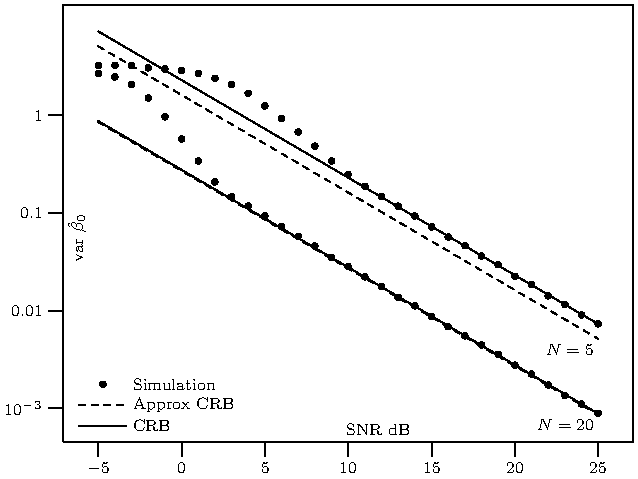
\includegraphics{code/data/plot-1-mps.pdf} 
    		\caption{Variance of $\hat{\beta}_0$ versus SNR.} 
    		\label{plot:phase0} 
 \end{figure} 

\clearpage

 \begin{figure}[p]
    	\centering 
   		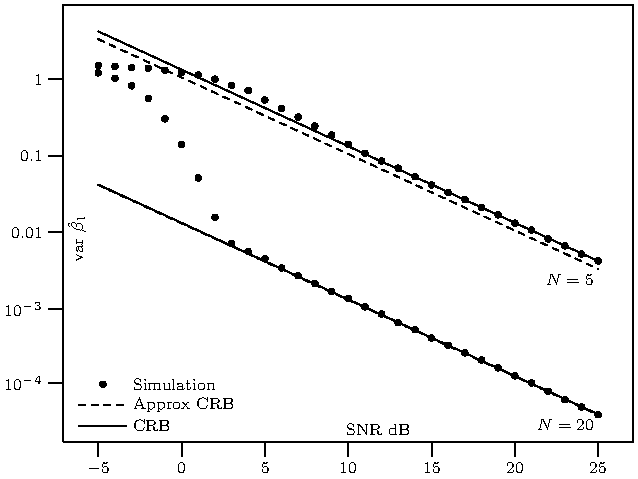
\includegraphics{code/data/plot-2-mps.pdf} 
    		\caption{Variance of $\hat{\beta}_1$ versus SNR.} 
    		\label{plot:phase1} 
 \end{figure} 

\clearpage

 \begin{figure}[p]
    	\centering 
   		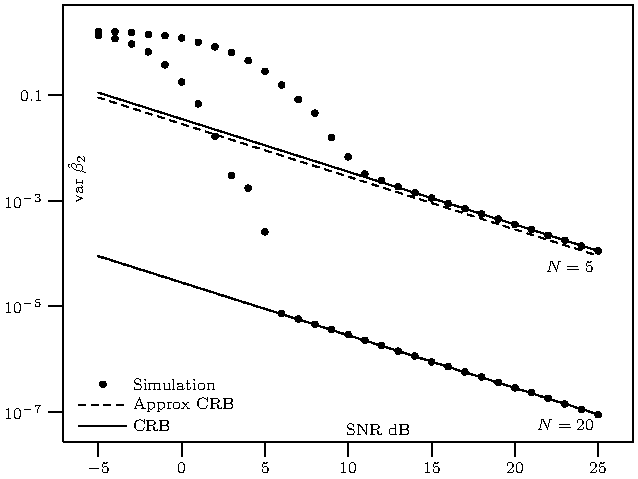
\includegraphics{code/data/plot-3-mps.pdf} 
    		\caption{Variance of $\hat{\beta}_2$ versus SNR.} 
    		\label{plot:phase2} 
 \end{figure}  
 
\clearpage

 \begin{figure}[p]
    	\centering 
   		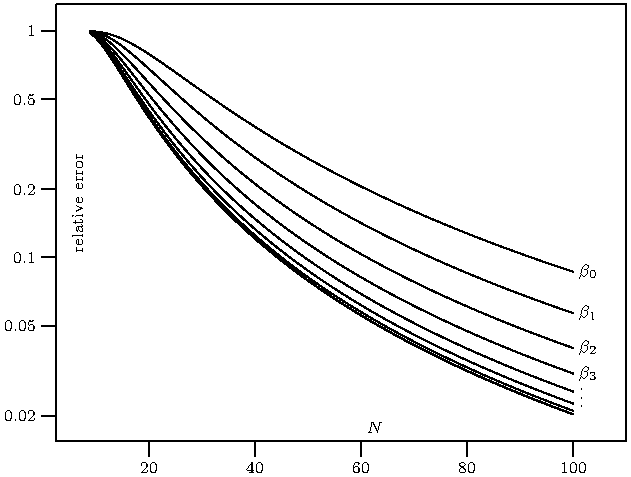
\includegraphics{code/data/plot-4-mps.pdf} 
    		\caption{Relative error of approximate Cram\'{e}r-Rao bound from~\cite{Peleg1991_CRB_PPS_1991} when $m=8$.} 
    		\label{plot:relerror} 
 \end{figure}

\end{document}